\chapter{Kajian Pustaka}
\label{chapter:kajian-pustaka}

Bab ini akan diisi oleh kajian pustaka yang berkaitan dengan topik persoalan tugas akhir untuk memberikan informasi mengenai dasar teori dan studi yang dipakai. Bab ini diharapkan dapat membantu pembaca untuk lebih mengerti tentang penelitian tugas akhir ini.

\section{Teknik \textit{Scaling} Basis Data Relasional}

Terdapat berbagai teknik umum yang digunakan untuk melakukan \textit{scaling} pada basis data relasional. Berikut adalah beberapa di antaranya:

\subsection{Replikasi basis data}

Replikasi berarti menyimpan salinan data yang sama pada beberapa mesin yang berbeda dan terhubung melalui jaringan \parencite{dataIntensiveApplications}. Terdapat beberapa alasan mengapa hal ini lazim dilakukan, yaitu:

\begin{enumerate}
    \item Untuk menjaga data tetap dekat secara geografis kepada pengguna, sehingga latensi berkurang.
    \item Agar sistem dapat terus berjalan meski terjadi kegagalan pada sebagian sistem, sehingga \textit{availability} meningkat.
    \item Untuk melakukan \textit{scale out} banyaknya mesin yang bisa melayani \textit{read queries}, sehingga meningkatkan \textit{read throughput}.
\end{enumerate}

Salah satu pendekatan yang umum diimplementasikan pada basis data relasional seperti PostgreSQL adalah replikasi berbasiskan \textit{leader and follower}. Satu \textit{node} ditugaskan sebagai \textit{leader} yang menerima operasi \textit{read and write}, lalu setiap perubahan yang terjadi akan direplikasi oleh replika (\textit{follower}). Dengan pola seperti ini, umumnya operasi \textit{write} hanya dapat ditangani oleh \textit{leader} dan operasi \textit{read} dapat ditangani oleh semua \textit{node}.

\begin{figure}[ht]
    \centering
    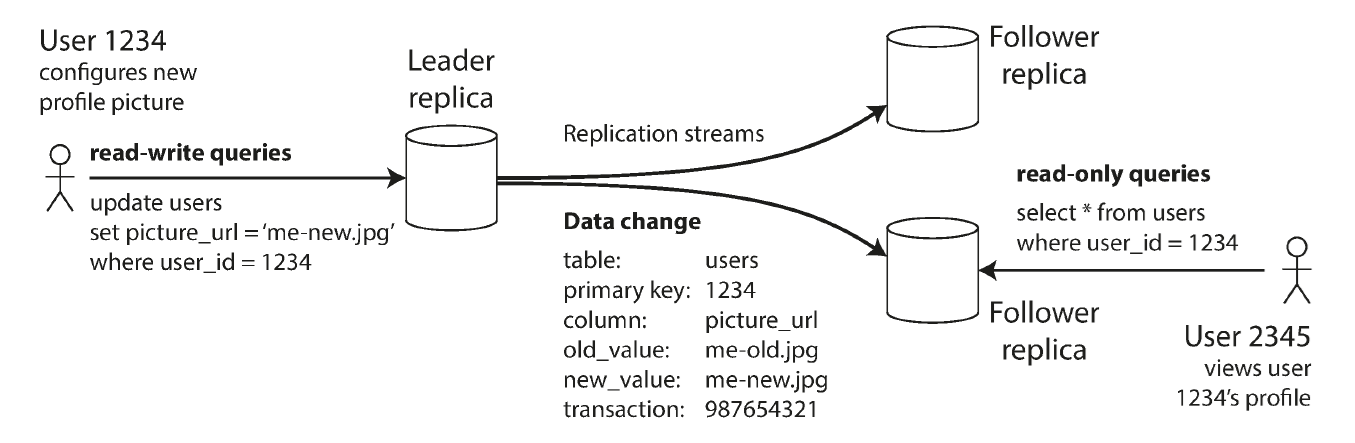
\includegraphics[width=0.8\textwidth]{resources/chapter-2/leader-based-replication.png}
    \caption{\textit{Leader-based (master-slave) replication \parencite{dataIntensiveApplications}}}
    \label{fig:leader-based-replication}
\end{figure}

Selain itu, proses replikasi juga terbagi menjadi dua, yaitu \textit{synchronous replication} dan \textit{asynchronous replication}. Pada \textit{synchronous replication}, data yang akan ditulis juga harus sudah ditulis oleh semua (atau mayoritas) replika sebelum dapat di-\textit{acknowledge}. Pada \textit{asynchronous replication}, data akan ditulis terlebih dahulu pada \textit{leader} lalu perubahannya dipropagasikan kepada \textit{replika}. Setiap pendekatan ini memiliki \textit{tradeoff} tersendiri. \textit{Synchronous replication} menjamin mayoritas \textit{node} memiliki data paling terbaru, tetapi latensi pada proses penulisan akan meningkat, sedangkan pada \textit{asynchronous replication} latensi penulisan jauh lebih kecil, tetapi data pada \textit{replica} menjadi \textit{eventually consistent}. Kedua mode replikasi ini didukung oleh PostgreSQL.

\section{Basis Data Relasional Terdistribusi}

\subsection{Citus: PostgreSQL Terdistribusi}

Citus merupakan mesin basis data terdistribusi untuk PostgreSQL yang menangani kebutuhan skalabilitas pada ekosistem PostgreSQL \parencite{citus}. Sebagai sebuah ekstensi, Citus menjaga kompatibilitas dengan PostgreSQL, sehingga dapat digunakan dengan PostgreSQL versi terbaru.

Sebuah kluster memiliki banyak \textit{node} yang terspesialisasi menjadi koordinator dan node pekerja. Aplikasi mengirimkan kueri kepada koordinator, lalu diteruskan kepada node pekerja terkait. Pendekatan ini memungkinkan setiap \textit{node} mampu memproses permintaan tulis sehingga pemrosesan bisa dilakukan secara parallel.

Selain itu, Citus memiliki skema \textit{sharding} berdasarkan skema dan baris. Hal ini diilustrasikan pada Gambar \ref{fig:row-vs-schema-sharding} yang membandingkan pemartisian rentang dan hash, menampilkan pertukaran antara kemudahan kueri rentang dengan distribusi beban yang merata.

\begin{figure}[H]
    \centering
    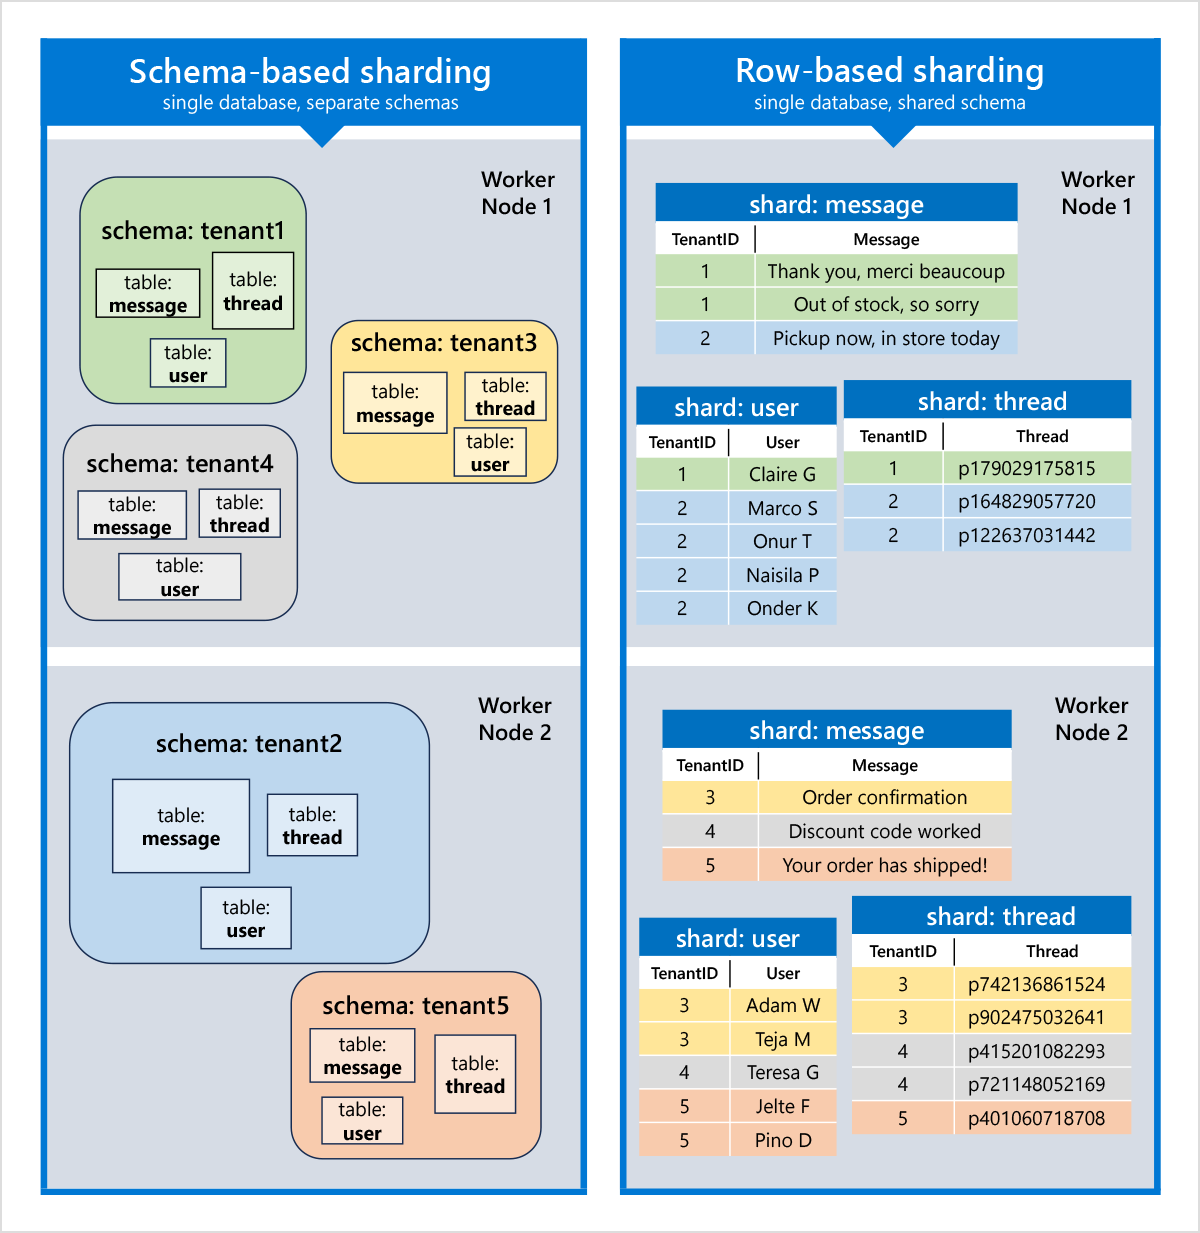
\includegraphics[width=0.8\textwidth]{resources/chapter-2/row-vs-schema-sharding.png}
    \caption{Perbandingan Pemartisian Data \parencite{schemaBasedSharding}}
    \label{fig:row-vs-schema-sharding}
\end{figure}

Selain itu, berikut adalah fitur lain ekstensi Citus:

\begin{enumerate}
    \item Tabel dibagi ke seluruh kluster node untuk menggabungkan sumber daya mesin (\textit{distributed tables}).
    \item Tabel referensi direplikasi ke seluruh node untuk kebutuhan penggabungan (\textit{join}) dan \textit{foreign key}, sehingga kinerja pembacaan data semakin baik (\textit{references tables}).
    \item Mesin kueri terdistribusi mengarahkan dan memparalelkan operasi pada tabel terdistribusi ke seluruh kluster.
    \item Model permartisian data berdasarkan baris dan berdasarkan skema.
\end{enumerate}


\subsection{YugaByteDB}

YugaByteDB merupakan basis data relasional terdistribusi dengan konsensus Raft. YugaByteDB memenuhi prinsip ACID dan terdistribusi secara \textit{native}. YugaByteDB kompatibel dengan API Cassandra (YCQL) dan API Postgres (YSQL).

YugaByteDB memanfaatkan pemartisian untuk mencapai ketersediaan tinggi dan toleransi kegagalan. Tablet yang berisi grup data direplikasi pada beberapa instans. Dengan begitu, penulisan dapat dilakukan pada instans yang berbeda dan operasi pembacaan dapat dilakukan pada banyak instans \parencite{yugabyteBaeldung}.

\begin{figure}[H]
    \centering
    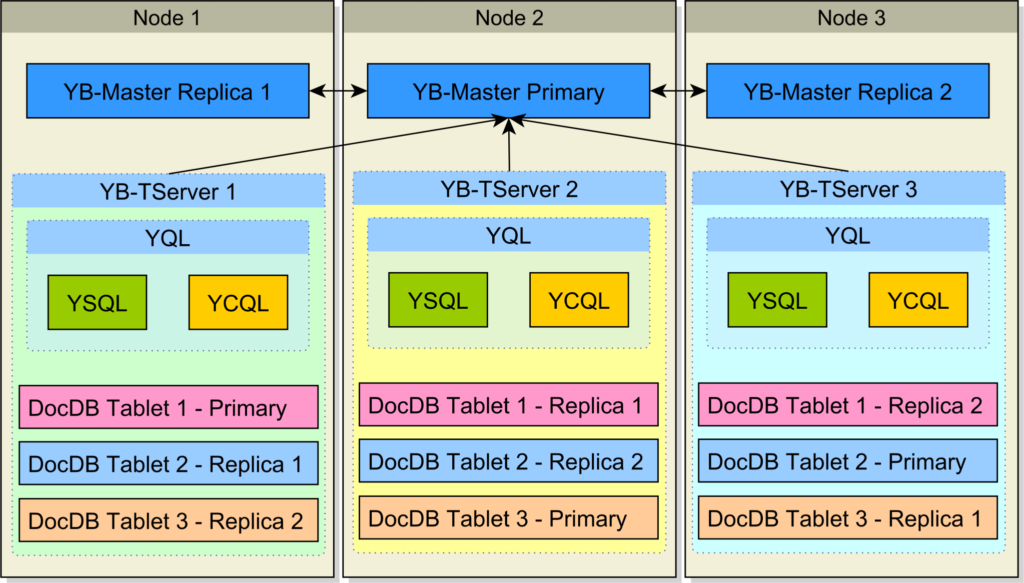
\includegraphics[width=0.8\textwidth]{resources/chapter-2/yugabyte.png}
    \caption{Arsitektur YugaByteDB \parencite{yugabyteBaeldung}}
    \label{fig:yugabyte-architecture}
\end{figure}

Gambar \ref{fig:yugabyte-architecture} menunjukkan arsitektur YugabyteDB dengan komponen Master dan TServer. Master mengelola metadata, sedangkan TServer menyimpan data. Ini relevan karena memperlihatkan bagaimana replikasi Raft digunakan.

\section{Pengendalian Aliran}

Sebuah layanan dalam satu sistem sering kali bertugas untuk mengerjakan sesuatu dan memanggil layanan lain. Dalam kasus ini, terdapat kemungkinan munculnya masalah kinerja dan keandalan ketika layanan mengalami beban yang tinggi. Keadaan ini dapat menciptakan situasi \textit{backpressure}.

Dalam konteks perangkat lunak, \textit{backpressure} dapat didefinisikan sebagai \textit{resistance or force opposing the desired flow of data through software} \parencite{backpressureExplained}. Selain melakukan penyesuaian pada sumber daya sistem, terdapat tiga strategi yang dapat digunakan untuk menangani \textit{backpressure}, yaitu:

\begin{enumerate}
    \item Mengurangi kecepatan produsen mengirimkan pesan.
    \item Menggunakan penyangga untuk sementara mengakumulasikan pesan.
    \item Membuang/menolak sebagian pesan yang diterima.
\end{enumerate}

Pola penyeimbangan beban berbasiskan antrean merupakan pola desain yang menyelesaikan masalah \textit{backpressure} dengan menggunakan antrean yang bertindak sebagai penyangga antara pesan dengan sebuah layanan, sehingga beban dapat dikontrol dan layanan tetap berjalan dengan stabil \parencite{queueLoadLeveling}.

\begin{figure}[H]
    \centering
    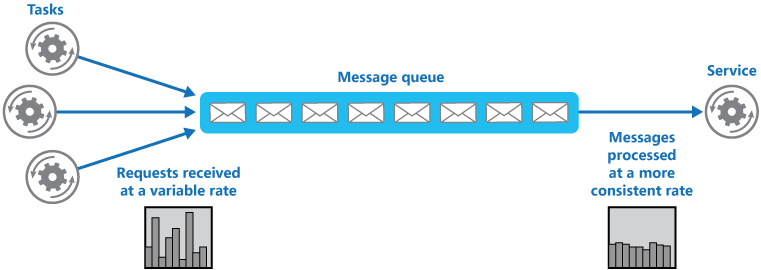
\includegraphics[width=0.8\textwidth]{resources/chapter-2/queue-based-load-leveling-pattern.png}
    \caption{Pola Penyeimbangan Beban Berbasiskan Antrean \parencite{queueLoadLeveling}}
    \label{fig:queue-based-load-leveling-pattern}
\end{figure}

Gambar \ref{fig:queue-based-load-leveling-pattern} memperlihatkan pola antrean sebagai mekanisme pengendalian aliran. Ini menunjukkan bagaimana antrean dapat menahan permintaan berlebih agar tidak langsung membebani layanan downstream. Penggunaan antrean memisahkan pesan dengan pekerja, sehingga pekerja dapat menangani pesan berdasarkan kemampuannya, terlepas dari banyaknya pekerjaan yang bertambah seiring dengan berjalannya waktu. Pola ini memiliki berbagai keuntungan, seperti menjaga ketersediaan, memaksimalkan skalabilitas, dan membatasi biaya atau penggunaan sumber daya. Meskipun begitu, penggunaan pola ini akan meningkatkan latensi, terlebih lagi apabila pesan yang dikirimkan jauh lebih besar daripada kapasitas pemrosesan pada sistem.

\subsection{Redis}

Redis (Remote Dictionary Service) merupakan basis data \textit{open-source} berbasiskan \textit{key-value store}. Redis mendukung berbagai tipe data, mulai dari string, bitmap, bitfield, hash, list, set, hingga stream. Selain itu, Redis merupakan basis data yang menyimpan data pada memori (\textit{in-memory}) dan berjalan secara \textit{single thread} sehingga Redis berjalan dengan cepat dan tidak perlu memikirkan konkurensi. Selain itu, Redis memiliki banyak dukungan fitur seperti dukungan \textit{persistence} dengan \textit{snapshot} atau \textit{append-only file} (AOF), dukungan \textit{high-availability}, replikasi, \textit{sharding}, \textit{pubsub}, \textit{stream}, dan lain-lain \parencite{redisExplained}.

\begin{figure}[htbp]
    \centering
    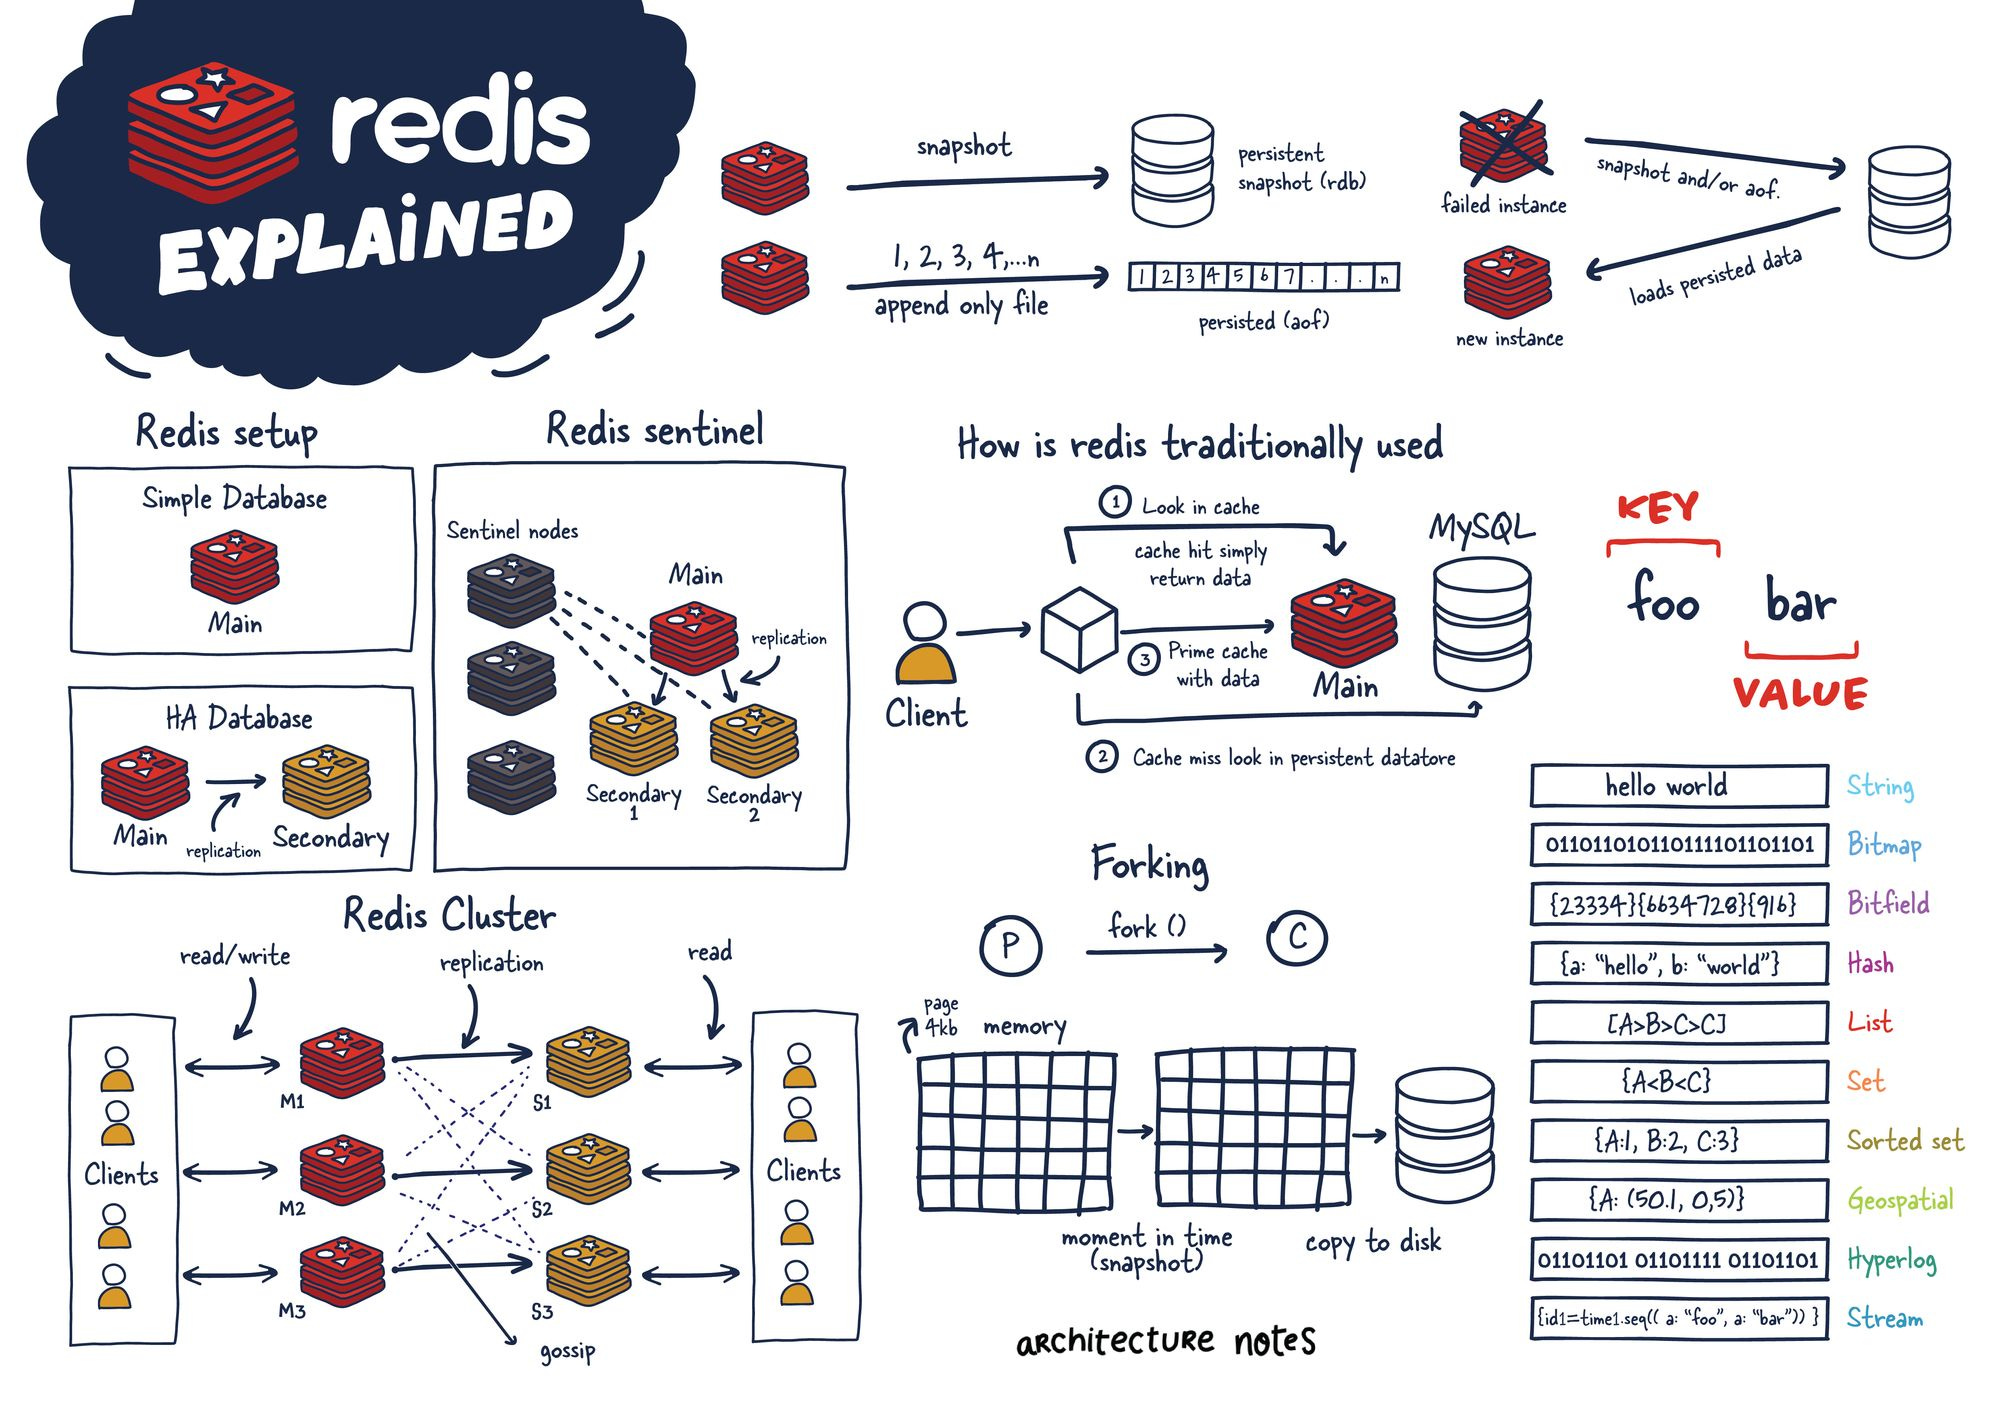
\includegraphics[width=1\textwidth]{resources/chapter-2/redis.jpg}
    \caption{\textit{Redis Explained \parencite{redisExplained}}}
    \label{fig:redis-explained}
\end{figure}

Konfigurasi Redis Cluster memungkinkan penskalaan secara horizontal dengan menyebarkan data pada mesin (\textit{sharding}). Redis menggunakan fungsi hash deterministik untuk mendistribusikan data. Selain itu, Redis menggunakan \textit{gossip protocol} untuk menilai keadaan kluster. Ketika \textit{master} tidak responsif, node \textit{secondary} dapat dipromosikan menjadi node \textit{primary} \parencite{redisExplained}.

\section{RabbitMQ}

RabbitMQ merupakan salah satu message broker yang engimplementasikan model penyimpanan berbasis antrean dan mendukung persistensi pesan baik secara persisten maupun tidak kekal. Dari segi performa, RabbitMQ memiliki throughput hingga 60 ribu pesan per detik dengan latensi tergolong rendah (dalam milidetik). Model konsumennya bersifat \textit{push-based}, artinya broker secara aktif mengirimkan pesan ke konsumen. Alur ini ditunjukkan pada Gambar \ref{fig:rabbitmq-flow}. RabbitMQ mendukung berbagai protokol seperti AMQP, MQTT, dan STOMP. Jaminan urutan pengiriman pesan pada RabbitMQ berlaku pada level antrean \parencite{arshadChoosingTheRightMessaging}.

\begin{figure}[htbp]
    \centering
    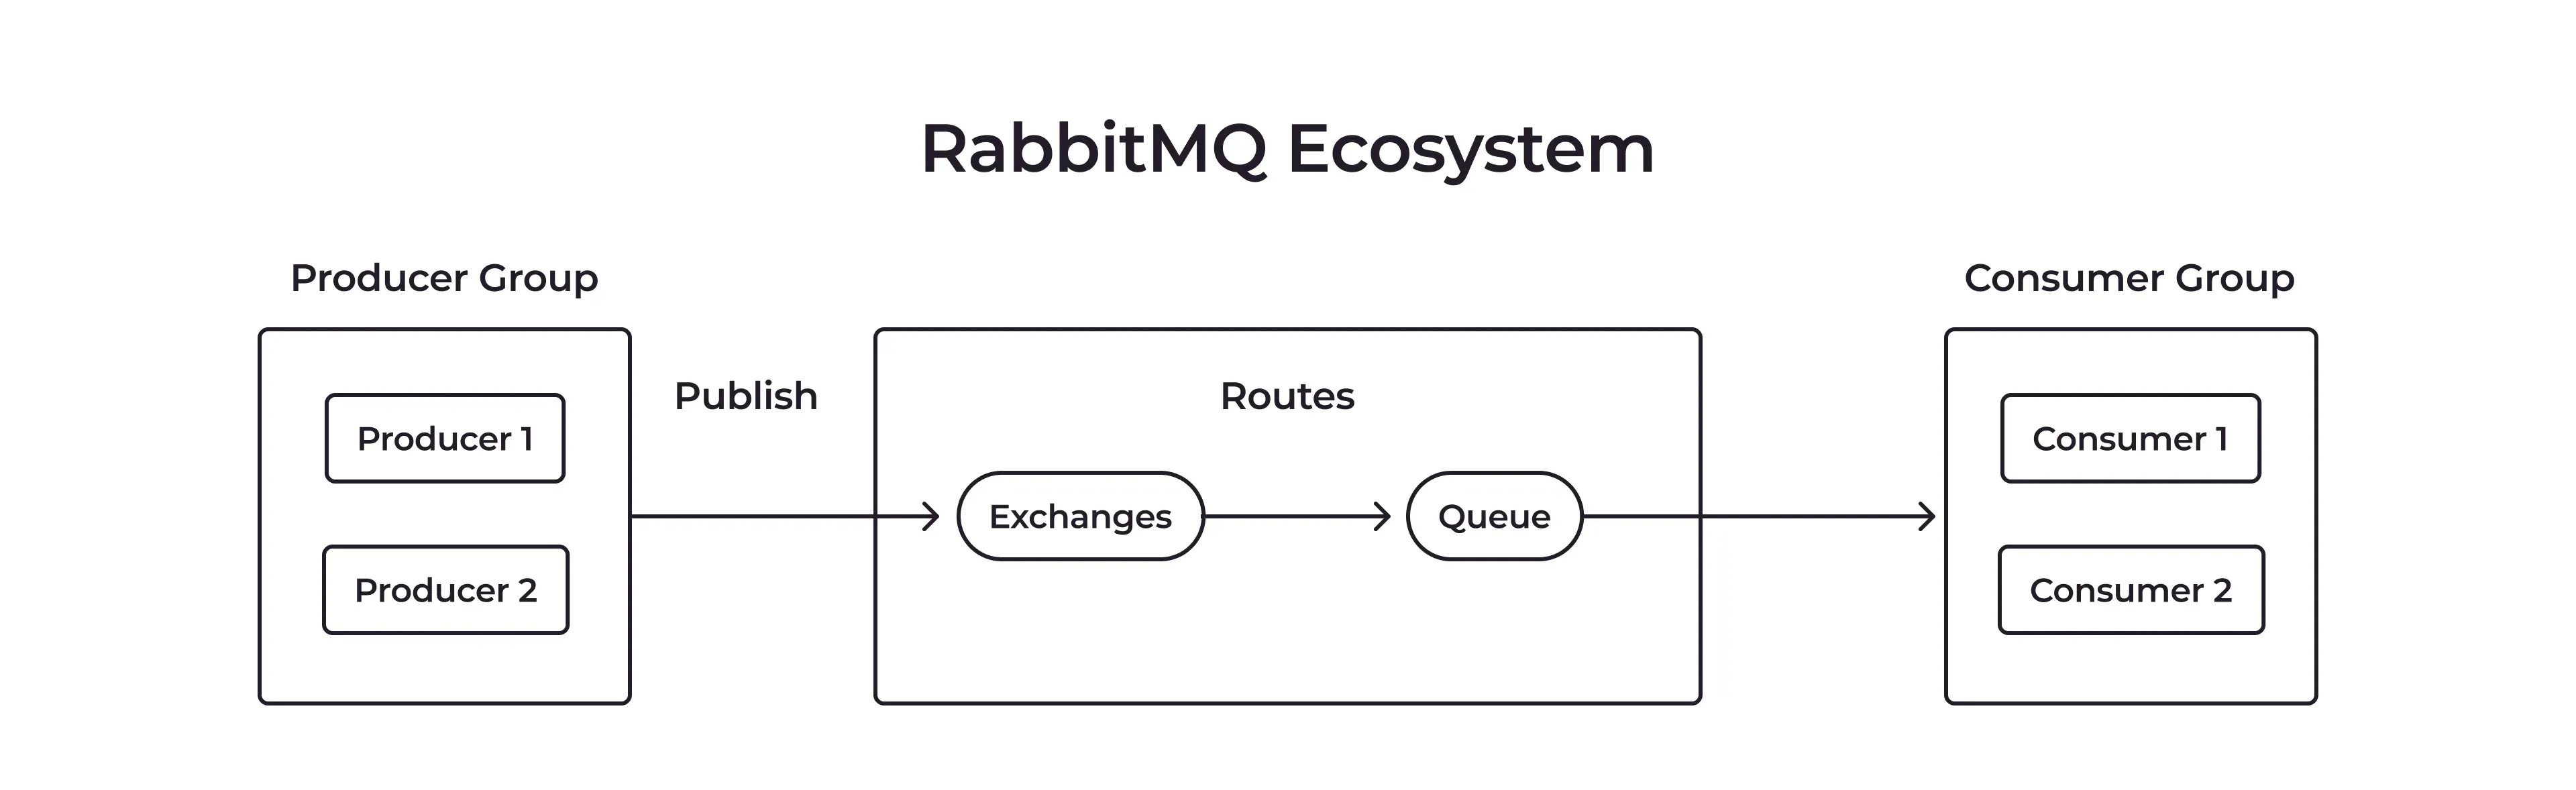
\includegraphics[width=0.8\textwidth]{resources/chapter-2/rabbitmq.jpeg}
    \caption{Alur RabbitMQ \parencite{royNatsRmqKafka}}
    \label{fig:rabbitmq-flow}
\end{figure}


\section{Penelitian dan Riset Terkait}

\subsection{Implementasi Arsitektur \textit{Microservices} Menggunakan Komunikasi \textit{Event-Driven} Pada Aplikasi Pemesanan Tiket Acara (Jeeves)}

Tugas akhir ini membahas aplikasi pemesanan tiket acara dengan arsitektur \textit{microservice} dengan komunikasi berbasis peristiwa. Tujuan dari penelitian tersebut adalah membuat aplikasi tiket yang tahan akan kegagalan sehingga layanan yang masih berjalan tetap dapat memenuhi aksi yang lain. Untuk itu, arsitektur \textit{microservice} diimplementasikan dengan cara \textit{loosely-coupled}. Agar hal tersebut dapat dipenuhi, komunikasi berbasis peristiwa digunakan. Agar ketergantungan antar layanan berkurang, seluruh data yang diperlukan oleh sebuah layanan diikutsertakan pada peristiwa yang dikirim \parencite{microservicesEventDriven}.

\begin{figure}[htbp]
    \centering
    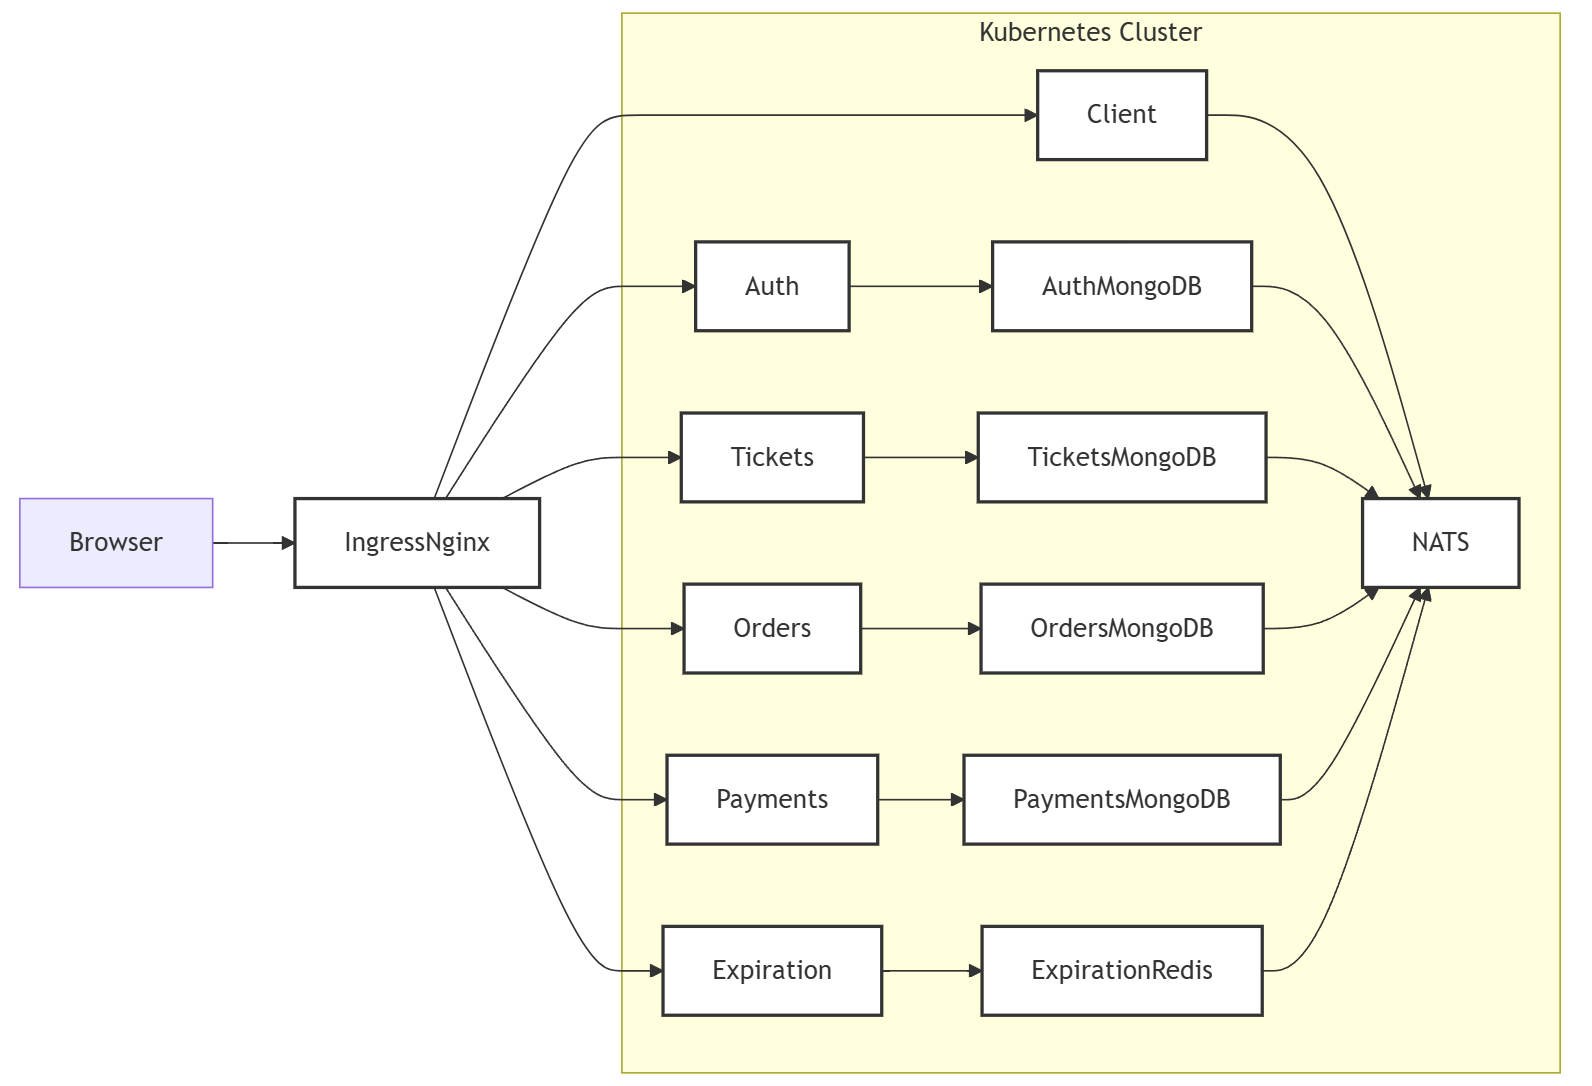
\includegraphics[width=1\textwidth]{resources/chapter-2/jeeves.png}
    \caption{Arsitektur Jeeves \parencite{microservicesEventDriven}}
    \label{fig:jeeves-architecture}
\end{figure}

Penelitian ini mengimplementasikan fungsionalitas dasar seperti otentikasi pengguna, pembuatan tiket, reservasi tiket, dan pembayaran tiket. Terdapat lima \textit{microservice} yang dibuat, yaitu layanan otentikasi, layanan tiket, layanan pemesanan, layanan pembayaran, dan layanan kadaluarsa. Setiap layanan selain layanan kadaluarsa memiliki basis data masing-masing dengan menggunakan MongoDB. Hanya layanan kadaluarsa yang menggunakan Redis. Selain itu, setiap komunikasi yang terjadi secara asinkron dilakukan melalui NATS. Untuk melakukan validasi otentikasi, sistem ini menggunakan JWT dengan rahasia bersama yang diatur oleh Kubernetes. Pendekatan ini memungkinkan layanan independen terhadap layanan otentikasi \parencite{microservicesEventDriven}.

Penelitian ini berhasil mengimplementasikan arsitektur aplikasi untuk pemesanan tiket acara yang tahan kegagalan dengan pendekatan \textit{microservice} dan berbasis peristiwa. Meskipun begitu, penelitian ini tidak membahas dan menguji aspek skalabilitas dan elastisitas dari sistem ini.

\subsection{\textit{Backend for a Ticketing System}}

Tesis ini membahas desain \textit{backend} untuk sistem tiket. Tesis ini berfokus pada desain modul, fungsionalitas, serta relasi yang diperlukan untuk menjalankan sistem ini. Penelitian ini berbeda dengan penelitian sebelumnya yang fokus membahas desain dari sisi arsitektur. Tesis ini tidak membahas arsitektur secara detil dan hanya membagi fungsionalitas menjadi beberapa modul. Oleh karena itu, arsitektur yang digunakan pada penelitian ini adalah arsitektur \textit{modular monolith}. Selain itu, penelitian ini memakai prinsip REST API dalam mendesain implementasi API \parencite{backendForTicketing}.

Terdapat empat entitas yang digambarkan pada sistem ini, yaitu:

\begin{enumerate}
    \item Pengguna yang bertugas untuk mencari dan membeli tiket, melakukan pembayaran, dan mengubah profil pengguna.
    \item Organisasi yang bertugas untuk mengatur acara, kategori tiket, dan lain-lain.
    \item Validator yang bertugas untuk memberi izin dan mencegah terjadinya pelanggaran yang berkaitan dengan validitas dan integritas tiket.
    \item Admin yang bertugas atas registrasi organisasi dan mengatur sertifikat penjual tiket.
\end{enumerate}

Figur \ref{fig:event-rm} dan \ref{fig:ticket-storage} menggambarkan diagram relasi entitas untuk \textit{events} dan entitas yang berkaitan pada proses pembuatan dan penyimpanan tiket.

\begin{figure}[htbp]
    \centering
    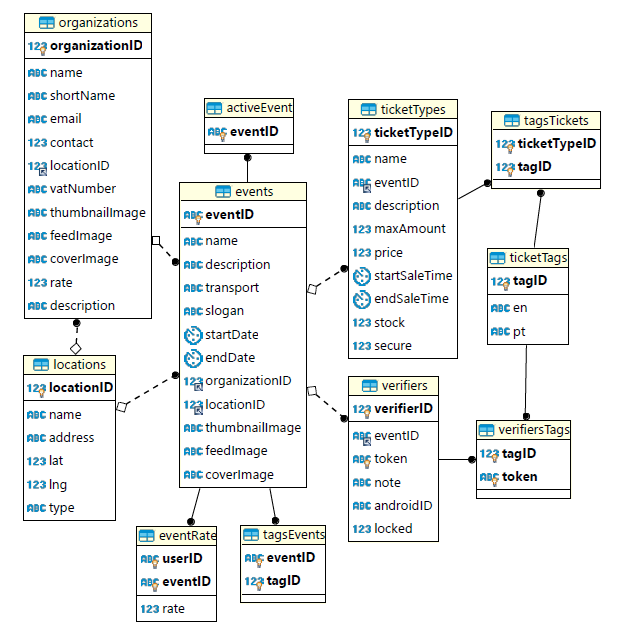
\includegraphics[width=0.6\textwidth]{resources/chapter-2/event-rm.png}
    \caption{ERD \textit{events} \parencite{backendForTicketing}}
    \label{fig:event-rm}
\end{figure}

\begin{figure}[htbp]
    \centering
    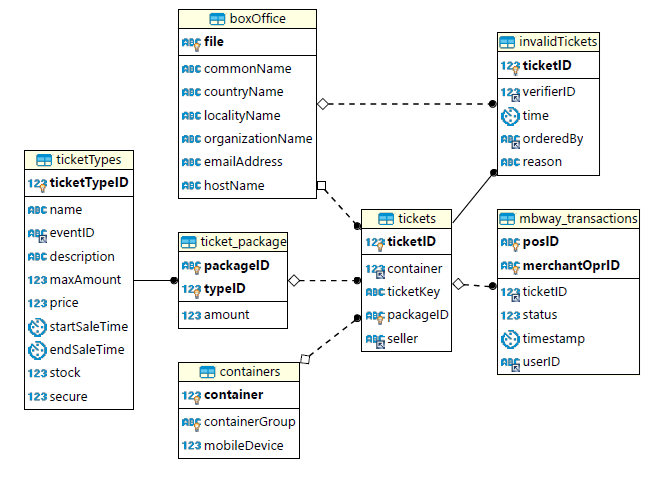
\includegraphics[width=0.6\textwidth]{resources/chapter-2/er-ticket-storage.png}
    \caption{ERD dengan entitas untuk pembuatan dan penyimpanan tiket \parencite{backendForTicketing}}
    \label{fig:ticket-storage}
\end{figure}

Sebagaimana dijelaskan sebelumnya, tesis ini hanya membahas sistem dari aspek desain fitur dan entitas. Arsitektur sistem tidak dibahas secara detil, sehingga kemungkinkan besar arsitektur yang diimplementasikan adalah arsitektur \textit{monolith}. Selain itu, aspek skalabilitas dan toleransi kegagalan tidak dibahas pada tesis ini.
